%%%%%%%%%%%%%%%%%%%%%%%%%%%%%%%%%%%%%%%%%%%%%%%%%%%%%%%%%%%%%%%%%%%%%%%%%%%%%%%%%%%%%%%%%%%%%%%%
%
% CSCI 1430 Written Question Template
%
% This is a LaTeX document. LaTeX is a markup language for producing documents.
% Your task is to answer the questions by filling out this document, then to
% compile this into a PDF document.
%
% TO COMPILE:
% > pdflatex thisfile.tex
%
% If you do not have LaTeX and need a LaTeX distribution:
% - Departmental machines have one installed.
% - Personal laptops (all common OS): http://www.latex-project.org/get/
%
% If you need help with LaTeX, come to office hours. Or, there is plenty of help online:
% https://en.wikibooks.org/wiki/LaTeX
%
% Good luck!
% James and the 1430 staff
%
%%%%%%%%%%%%%%%%%%%%%%%%%%%%%%%%%%%%%%%%%%%%%%%%%%%%%%%%%%%%%%%%%%%%%%%%%%%%%%%%%%%%%%%%%%%%%%%%
%
% How to include two graphics on the same line:
%
% \includegraphics[width=0.49\linewidth]{yourgraphic1.png}
% \includegraphics[width=0.49\linewidth]{yourgraphic2.png}
%
% How to include equations:
%
% \begin{equation}
% y = mx+c
% \end{equation}
%
%%%%%%%%%%%%%%%%%%%%%%%%%%%%%%%%%%%%%%%%%%%%%%%%%%%%%%%%%%%%%%%%%%%%%%%%%%%%%%%%%%%%%%%%%%%%%%%%

\documentclass[11pt]{article}

\usepackage[english]{babel}
\usepackage[utf8]{inputenc}
\usepackage[colorlinks = true,
            linkcolor = blue,
            urlcolor  = blue]{hyperref}
\usepackage[a4paper,margin=1.5in]{geometry}
\usepackage{stackengine,graphicx}
\usepackage{fancyhdr}
\setlength{\headheight}{15pt}
\usepackage{microtype}
\usepackage{times}
\usepackage[shortlabels]{enumitem}
\setlist[enumerate]{topsep=0pt}
% python code format: https://github.com/olivierverdier/python-latex-highlighting
\usepackage{pythonhighlight}

\frenchspacing
\setlength{\parindent}{0cm} % Default is 15pt.
\setlength{\parskip}{0.3cm plus1mm minus1mm}

\pagestyle{fancy}
\fancyhf{}
\lhead{Project 3 Questions}
\rhead{CSCI 1430}
\rfoot{\thepage}

\date{}

\title{\vspace{-2cm}Project 3 Questions}


\begin{document}
\maketitle
\thispagestyle{fancy}
\vspace{-3cm}

\section*{Instructions}
\begin{itemize}
  \item 6 questions.
  \item Write code where appropriate; feel free to include images or equations.
  \item Please make this document anonymous.
  \item This assignment is \textbf{fixed length}, and the pages have been assigned for you in Gradescope. As a result, \textbf{please do NOT add any new pages}. We will provide ample room for you to answer the questions. If you \emph{really} wish for more space, please add a page \emph{at the end of the document}.
  \item \textbf{We do NOT expect you to fill up each page with your answer.} Some answers will only be a few sentences long, and that is okay.
\end{itemize}

\section*{Questions}

%%%%%%%%%%%%%%%%%%%%%%%%%%%%%%%%%%%

\paragraph{Q1:} 

\begin{enumerate} [(a)]
    \item Define these common terms in machine learning:
    \begin{enumerate} [(i)]
    \item Bias
    \item Variance
    \end{enumerate}
    \item Define these terms in the context of evaluating a classifier:
    \begin{enumerate} [(i)]
    \item Overfitting
    \item Underfitting
    \end{enumerate}
    \item How do overfitting and underfitting relate to bias and variance?
\end{enumerate}

\emph{Please answer overleaf.}

%%%%%%%%%%%%%%%%%%%%%%%%%%%%%%%%%%%
\pagebreak
\paragraph{A1:} Your answer here.
% Uncomment the stencil below and fill in your solution.

% \begin{enumerate}[(a)]

% \item 
%     \begin{enumerate} [(i)]
%     \item 
%     \item
%     \end{enumerate}

% \item 
%     \begin{enumerate} [(i)]
%     \item 
%     \item
%     \end{enumerate}
% \item 

% \end{enumerate}


%%%%%%%%%%%%%%%%%%%%%%%%%%%%%%%%%%%

\pagebreak
\paragraph{Q2:} Suppose we create a visual word dictionary using SIFT and k-means clustering for a scene recognition algorithm. Examining the SIFT features generated from our training database, we see that many are almost equidistant from two or more visual words. 
\begin{enumerate}[(a)]
    \item 
    Why might this affect classification accuracy?

    \item
    Given the situation, describe \emph{two} methods to improve classification accuracy, and explain why they would help.\\ 
    \emph{These can be for k-means, or otherwise.}

\end{enumerate}


%%%%%%%%%%%%%%%%%%%%%%%%%%%%%%%%%%%
\paragraph{A2:} Your answer here.
% Uncomment the stencil below and fill in your solution.

% \begin{enumerate}[(a)]

% \item 

% \item 

% \end{enumerate}



%%%%%%%%%%%%%%%%%%%%%%%%%%%%%%%%%%%

\pagebreak
\paragraph{Q3:} The way that the bag of words representation handles the spatial layout of visual information can be both an advantage and a disadvantage.
\begin{enumerate}[(a)]
\item Describe an example scenario for each of these cases.
\item Describe a modification or additional algorithm which might\\overcome the disadvantage.

\item How might we determine whether bag of words is a good model?
\end{enumerate}
%%%%%%%%%%%%%%%%%%%%%%%%%%%%%%%%%%%
\paragraph{A3:} Your answer here.
% Uncomment the stencil below and fill in your solution.

% \begin{enumerate}[(a)]

% \item 

% \item 

% \item 

% \end{enumerate}




%%%%%%%%%%%%%%%%%%%%%%%%%%%%%%%%%%%

\pagebreak
\paragraph{Q4:}
Evaluating whether a model is good can have huge impacts in deploying technologies. With companies inching their way towards full vehicle autonomy, questions of when and how the technology can be launched are deeply tied to model evaluation. 

\begin{enumerate}[(a)]
\item When deciding whether a self driving vehicle is fit for public roads, what accuracy would you consider to be ``good enough''?  (3-5 sentences)

\emph{Consider this question from the perspective of many people: a purchaser of the vehicle, a resident of the city where the vehicles will be released, an engineer on the team behind the vehicle, or a government regulator deciding whether they should be allowed.}

\item In the event that a self driving car makes an error and causes a crash, who is responsible? Why? (2-4 sentences)

\item The question of ``when is good enough?'' extends to many different computer vision applications. Beyond self-driving vehicles, please think of or find another real world example, and describe how this question might have or has had an effect.
\end{enumerate}

\emph{Please answer overleaf.}

%%%%%%%%%%%%%%%%%%%%%%%%%%%%%%%%%%%
\pagebreak
\paragraph{A4:} Your answer here.
% Uncomment the stencil below and fill in your solution.

% \begin{enumerate}[(a)]

% \item 

% \item 

% \item 

% \end{enumerate}

%%%%%%%%%%%%%%%%%%%%%%%%%%%%%%%%%%%



%%%%%%%%%%%%%%%%%%%%%%%%%%%%%%%%%%%
\pagebreak
\paragraph{Q5:} Given a linear classifier such as SVM which separates two classes (binary decision), how might we use multiple linear classifiers to create a new classifier which separates $k$ classes?

Below, we provide pseudocode for a linear classifier. It trains a model on a training set, and then classifies a new test example into one of two classes. Please edit the pseudo-code to convert this into a multi-class classifier. 

\emph{Hints:} See slides in supervised learning crash course deck, plus your own research. You can take either the one vs.~all (or one vs.~others) approach or the one vs.~one approach in the slides; please declare which approach you take.

\emph{More hints:} Be aware that 1) the input labels in the multi-class case are different, and you will need to match the expected label input for the \texttt{train\_linear\_classifier} function, 2) you need to make a new decision on how to aggregate or decide on the most confident prediction.

\emph{Note:} A more efficient software application would separate the classifier training and testing into two different functions so that the model could be reused without retraining. Feel free to ignore this for now.

\emph{Please answer overleaf.}

%%%%%%%%%%%%%%%%%%%%%%%%%%%%%%%%%%%
\pagebreak
\paragraph{A5:} Your answer here.

\begin{python}
# Inputs
#   train_feats: N x d matrix of N features each d descriptor long
#   train_labels: N x 1 array containing values of either -1 (class 0) or 1 (class 1)
#   test_feat: 1 x d image for which we wish to predict a label
#
# Outputs
#   -1 (class 0) or 1 (class 1)
#
# Please turn this into a multi-class classifier for k classes.
# Inputs:
#    As before, except
#    train_labels: N x 1 array of class label integers from 0 to k-1
# Outputs:
#    A class label integer from 0 to k-1
#
def classify(train_feats, train_labels, test_feat)
    # Train classification hyperplane
    weights, bias = train_linear_classifier(train_feats, train_label)
    # Compute distance from hyperplane
    test_score = weights * test_feats + bias

    return 1 if test_score > 0 else -1
\end{python}
% %%%%%%%%%%%%%%%%%%%%%%%%%%%%%%%%%%%


% %%%%%%%%%%%%%%%%%%%%%%%%%%%%%%%%%%%
\pagebreak

\paragraph{Q6:} When performing HOG, the parameters such as pixels per cell and cells per block can greatly impact the resulting feature descriptor, thereby affecting your models' performance on a classification task. Please answer the following questions using this diagram for reference.

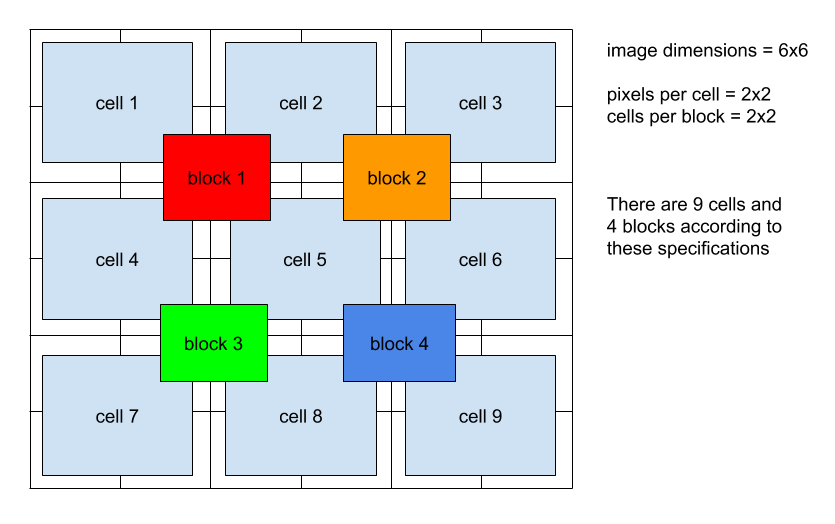
\includegraphics[width=\textwidth]{hog-diagram.png}

\emph{Note:} There is a feature descriptor for each block. Since HOG outputs a histogram of size 9 per cell, you can append those together to get the feature descriptor for each block. As a result of this, if you have (z,z) cells per block, the feature descriptor for each block will be of size z*z*9.

\emph{Note:} The blocks are overlapping as displayed in the diagram.

\begin{enumerate}[(a)]
\item Given an image of dimmensions 72x72, calculate the number of cells, blocks, and feature vector size that will occur if performing hog with the following parameters.

Scenario 1: pixels per cell = 4x4, cells per block = 4x4 (like your implementation of SIFT!)
\\ 
Number of cells: 
\\
Number of blocks: 
\\
Dimensions of resulting feature descriptor: 
\\

Scenario 2: pixels per cell = 8x8, cells per block = 2x2
\\ 
Number of cells:
\\
Number of blocks: 
\\
Dimensions of resulting feature descriptor: 


\item What are the pros and cons of the two parameter combinations? Which might you expect to have better performance?

\emph{Note:} You might find it useful to look at this paper (http://lear.inrialpes.fr/people/dalal/NavneetDalalThesis.pdf) on pages 39, 41
\end{enumerate}

\emph{Please answer overleaf.}

%%%%%%%%%%%%%%%%%%%%%%%%%%%%%%%%%%%
\pagebreak
\paragraph{A6:} Your answer here.
% Uncomment the stencil below and fill in your solution.

% \begin{enumerate}[(a)]

% \item 

% \item  

% \end{enumerate}

%%%%%%%%%%%%%%%%%%%%%%%%%%%%%%%%%%%



% %%%%%%%%%%%%%%%%%%%%%%%%%%%%%%%%%%%
% \pagebreak
% \paragraph{Secret something to think about:} Given a linear classifier like SVM, how might we handle data that are not linearly separable? How does the \emph{kernel trick} help in these cases? 

% \emph{Hint: See slides in supervised learning crash course deck, plus your own research.}

% %%%%%%%%%%%%%%%%%%%%%%%%%%%%%%%%%%%
% \paragraph{A:} Your answer here.



%%%%%%%%%%%%%%%%%%%%%%%%%%%%%%%%%%%
\pagebreak
\section*{Feedback? (Optional)}
Please help us make the course better. If you have any feedback for this assignment, we'd love to hear it!


% \pagebreak
% \section*{Any additional pages would go here.}


\end{document}
